% Autor: Leonhard Segger, Alexander Neuwirth
% Datum: 2017-10-30
\documentclass[
	% Papierformat
	a4paper,
	% Schriftgröße (beliebige Größen mit „fontsize=Xpt“)
	12pt,
	% Schreibt die Papiergröße korrekt ins Ausgabedokument
	pagesize,
	% Sprache für z.B. Babel
	ngerman
]{scrartcl}

% Achtung: Die Reihenfolge der Pakete kann (leider) wichtig sein!
% Insbesondere sollten (so wie hier) babel, fontenc und inputenc (in dieser
% Reihenfolge) als Erstes und hyperref und cleveref (Reihenfolge auch hier
% beachten) als Letztes geladen werden!

% Silbentrennung etc.; Sprache wird durch Option bei \documentclass festgelegt
\usepackage{babel}
% Verwendung der Zeichentabelle T1 (Sonderzeichen etc.)
\usepackage[T1]{fontenc}
% Legt die Zeichenkodierung der Eingabedatei fest, z.B. UTF-8
\usepackage[utf8]{inputenc}
% Schriftart
\usepackage{lmodern}
% Zusätzliche Sonderzeichen
\usepackage{textcomp}

% Mathepaket (intlimits: Grenzen über/unter Integralzeichen)
\usepackage[intlimits]{amsmath}
% Ermöglicht die Nutzung von \SI{Zahl}{Einheit} u.a.
\usepackage{siunitx}
% Zum flexiblen Einbinden von Grafiken (\includegraphics)
\usepackage{graphicx}
% Abbildungen im Fließtext
\usepackage{wrapfig}
% Abbildungen nebeneinander (subfigure, subtable)
\usepackage{subcaption}
% Funktionen für Anführungszeichen
\usepackage{csquotes}
% Zitieren, Bibliographie
\usepackage{biblatex}


% Zur Darstellung von Webadressen
\usepackage{url}
%chemische Formeln
\usepackage[version=4]{mhchem}
% siunitx: Deutsche Ausgabe, Messfehler getrennt mit ± ausgeben
\usepackage{floatrow}
\floatsetup[table]{capposition=top}
\usepackage{float}
% Verlinkt Textstellen im PDF-Dokument
\usepackage[unicode]{hyperref}
% "Schlaue" Referenzen (nach hyperref laden!)
\usepackage{cleveref}
\sisetup{
	locale=DE,
	separate-uncertainty
}
\bibliography{6Mi_E2_10-01-2018_References}

\begin{document}
	
	\begin{titlepage}
		\centering
		{\scshape\LARGE Versuchsbericht zu \par}
		\vspace{1cm}
		{\scshape\huge E2 - Millikan \par}
		\vspace{2.5cm}
		{\LARGE Gruppe 6Mi \par}
		\vspace{0.5cm}
		
		{\large Alexander Neuwirth (E-Mail: a\_neuw01@wwu.de) \par}
		{\large Leonhard Segger (E-Mail: l\_segg03@uni-muenster.de) \par}
		\vfill
		
		durchgeführt am 10.01.2018\par
		betreut von\par
		{\large Johann Preuß}
		
		\vfill
		
		{\large \today\par}
	\end{titlepage}
	\tableofcontents
	\newpage
	
	\section{Kurzfassung}
	%TODO Hypothese	und deren Ergebnis
	%TODO Ergebnisse, auch Zahlen, mindestens wenn's halbwegs Sinn ergibt
	%TODO Was wurde gemacht
	%TODO Rechtschreib mal gucken, weil nur so gefreestyled (@myself)
	Durch den Millikan Versuch soll die Elemtentarladung bestimmt werden.
	Dies gelingt dadurch, dass man die Bewegung von Öltröpfchen in einem konstantem elektrischen Feld beobachtet.
	Einfluss auf die Bewegung nimmt die Gravitation, Luftreibung, Coulomb-Kraft und der Auftrieb.
	Da ein direktes Vermessen des Öltröpfchens nicht praktikabel ist, werden zwei Fälle untersucht.

	Erst wird die Zeit für eine bestimmte Strecke gemessen, wobei das elektrische Feld parallel zum Gravitationsfeld ausgerichtet ist. 
	Im zweiten Fall ist das elektrische Feld ausgeschaltet, sodass sich aus beiden Messugen Ladung und Radius des Tröpfchens bestimmen lassen.
	Die Ladung der Öltröpfchen entsteht durch Reibung beim Einsprühen in den Kondensator. 
	Die Hypothese lautet, dass wenn es eine Elementarladung gibt, müssten die Tröpfchen stets mit einem Vielfachen derer geladen sein. 
	%TODO Hypothese e- Theorie wert
	%TODO ERgebnisse
	%TODO mehr? 


	\section{Vorüberlegungen}
	Zur Vorbereitung auf den Versuch wurden folgende Aufgaben bearbeitet:
	\begin{itemize}
		\item Eine Skizze der Kräftegleichgewichte wurde vor dem Experiment angezeichnet und besprochen. In \cref{fall} und \cref{steig} sind diese dargestellt.
		\item Herleitung der Kräftegleichgewichte aus den Formeln für $ r $ und $ Q $: \\
		Die relevanten Kräftegleichgewichte lauten:
		\begin{align*}
			F_\text{G}=F_\text{R}+F_\text{A}\\
			F_\text{G}+F_\text{R}=F_\text{el}+F_\text{A}
		\end{align*}
		Wenn man hier die vorgegebenen Kräfte bei Öltröpfchen in Luft einsetzt, erhält man:
		\begin{align*}
			\frac{4}{3}\pi r^3 \rho_\text{Öl} g = 6 \pi \eta r v_\downarrow + \frac{4}{3}\pi r^3 \rho_\text{L}g\\
			\frac{4}{3}\pi r^3 \rho_\text{Öl} g + 6 \pi \eta r v_\uparrow = \frac{QU}{d} + \frac{4}{3}\pi r^3 \rho_\text{L}g
		\end{align*}
		Aus diesem Gleichungssystem erhält man nach einigen Umformungsschritten:
		\begin{align*}
			Q&=\frac{18 \pi d}{U} \sqrt{\frac{\eta^3 v_\downarrow}{2(\rho_\text{Öl}-\rho_\text{L})g}}(v_\downarrow + v_\uparrow)\\
			r&=3\sqrt{\frac{\eta v_\downarrow}{2(\rho_\text{Öl}-\rho_\text{L})g}}
		\end{align*}
		
		\item Die Dauer der Beschleunigungsphase der Tröpfchen muss nicht berücksichtigt werden, da die Fall- und Steiggeschwindigkeiten in der Größenordnung von \SI{E-4}{\meter \per \second} liegen, es also zu erwarten ist, dass die Beschleunigungsphase der Teilchen sehr kurz ist. 
		\item Es ist wichtig die Kondensatorplatten waagerecht auszurichten, weil sie einerseits parallel zu einander sein müssen, damit das elektrische Feld möglichst homogen ist und andererseits muss die Kraft des elektrischen Feldes parallel zur Gravitationskraft und damit allen anderen Kräften sein.
		\item Es werden Öltröpfchen anstelle von Wassertröpfchen verwendet, weil Öl deutlich weniger flüchtig ist, man also keinen Massenverlust der Tröpfchen während der Beobachtung mit einbeziehen muss.
		\item Im elektrischen Feld steigen stärker geladene Teilchen schneller auf als weniger geladene. Deshalb muss man, um stärker und weniger stark geladene Teilchen bei gleicher Geschwindigkeit zu beobachten, bei stärker geladenen Teilchen die Spannung verringern und umgekehrt sie bei schwächer geladenen erhöhen.
		\item Man sollte die einzelnen Messungen nicht innerhalb der Stoppuhr aufsummieren, weil dies bedeuten würde, dass wenn man sich bei einer der Messungen vermisst, alle bisherigen Messungen dieses Teilchens wiederholen müsste, während man ansonsten nur die eine misslungene erneut durchführen muss.
		\item Bei steigender Temperatur steigen mittlere Weglänge $ \lambda $ und Viskosität $ \eta $ in Luft (siehe Literaturwerte aus der Anleitung). %TODO Amazon-Reflink in der Videobeschreibung
		Dies ist nicht in allen Medien der Fall.
	\end{itemize}
	\begin{figure}[H]
		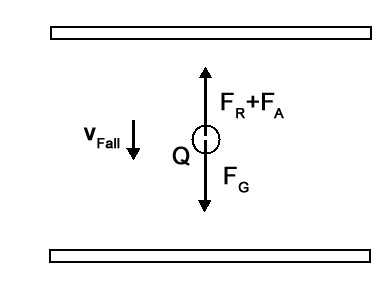
\includegraphics[width=0.4\textwidth]{fall}
		\centering
		\caption{Kräfte auf das Öltröpfchen während der Fallbewegung. Das elektrische Feld ist ausgeschaltet.\cite{RCL}}
		\label{fall}
		\centering
	\end{figure} 
	\begin{figure}[H]
		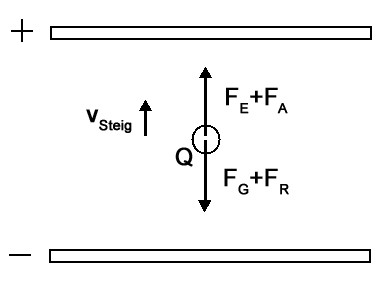
\includegraphics[width=0.4\textwidth]{steig}
		\centering
		\caption{Kräfte auf das Öltröpfchen während der Steigbewegung.\cite{RCL}}
		\label{steig}
		\centering
	\end{figure} 
	\section{Methoden}
	%TODO Bilder von der Website klauen
	In \cref{Millikan} ist er Aufbau des Experiments illustriert.
	Um die Öltröpfchen erkennbar zu machen wurde der Raum abgedunkelt und die Beleuchtungseinrichtung eingeschaltet.
	Zunächst wurden an den Kondensatorplatten mit einem Abstand $d$ eine Gleichspannung von ca. \SI{600}{V} angelegt. 
	Darauf wurden Öltröpfchen in das elektrische Feld gesprüht.
	Mit einem Mikroskop war nun erkennbar, dass ein Töpfchen welches ansteigt, geladen ist. 
	Durch die Linsen des Mikroskops ist das Bild seitenverkehrt, folglich hatte es den Anschein das Öltropfchen bewege sich nach unten. 
	Nachdem man eine Tröpfchen gefunden hatte, wurde das Feld ausgeschaltet und die Zeit gemessen die das Tröpfchen für eine Fall von zwei Skalenteilen (\SI{2}{mm}) benötigte. (Fallzeit)
	Dann wurde das elektrische Feld wieder eingeschaltet und dieselbe Messung wurde erneut durchgeführt mit umgekehrter Bewegung des Teilchens. (Steigzeit)
	Diese zwei Messungen wurden fünffach für 15 Tröpfchen durchgeführt. 
	Zu Beachten galt es, dass Luftstömungen die Tröpfchen beeinflussen können, desshalb wurde der Raum zwischen den Kondensatorplatten mit einem Stück Pappier zwischen Ölzerstäuber und Einsprühöffnung abgeschlossen.
	Außerdem steigt der Fehler mit der Ladung $Q$, wesshalb man bereits während des Experiments die Ladung einzelner Tröpfchen berechnet, um diese möglichst klein halten zu können.
	%TODO mehr!


	\begin{figure}[H]
		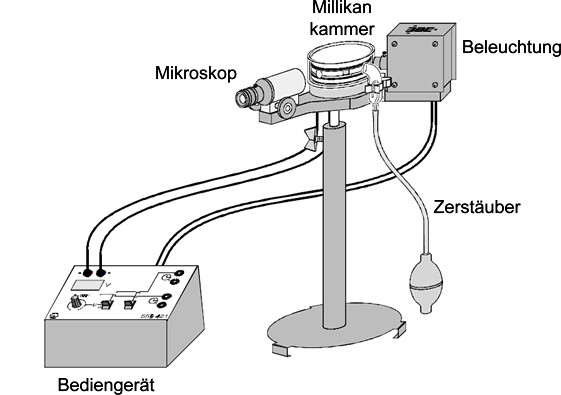
\includegraphics[width=0.7\textwidth]{Millikan}
		\centering
		\caption{Exemplarischer Aufbau des Millikan Versuchs.\cite{TUM} }
		\label{Millikan}
		\centering
	\end{figure} 

	
	\section{Ergebnisse und Diskussion}
	%TODO Datenanalyse -> Überschrift?
	%TODO Unsicherheiten
	

	\subsection{Beobachtung}
	\subsubsection*{Technische Daten und Konstanten} %TODO Amazon-Reflink in der Videobeschreibung
	\begin{itemize}
		\item Plattenabstand: $d=\SI{6 \pm 0,05}{mm}$
		\item Okularvergrößerung: 10
		\item Objektivvergrößerung: \SI{2 \pm 0,05}{}
		\item Länge der Mikrometerskala: \SI{10}{mm}
		\item kleine Skalenteilung: \SI{0,1}{mm}
		\item Öldichte: $\rho_\text{Öl} = \SI{874 \pm 1,2}{\kilogram \per \metre \cubed} $ (gemäß der Temperaturabhängigkeit der Dichte bei unbekannter exakter Temperatur nahe Raumtemperatur von \SI{20}{\degreeCelsius}mit rechteckiger WDF)
		\item Dynamische Viskosität der Luft: $\eta = \SI{18,2 \pm 0,18}{\micro \pascal \second} $ (gemäß der Temperaturabhängigkeit der Dynamischen Viskosität bei unbekannter exakter Temperatur nahe Raumtemperatur von \SI{20}{\degreeCelsius} mit rechteckiger WDF)
		\item Dichte der Luft: $\rho_\text{L}= \SI{1,2929}{\kilogram \per \metre \cubed}$ (ohne Unsicherheit, denn gering gegenüber der Dichte von Öl und deren Unsicherheit)
		\item Ortsfaktor: \SI{9,81 \pm 0,02}{\meter \per \second \squared} (ortsabhänige Schwankung nach oben abgeschätzt)
	\end{itemize}
	Die Spannung zwischen den Kondensatorplatten wurde auf \SI{565}{V} eingestellt, sank aber während des Versuchs auf \SI{560}{V}.
	Die Unsicherheit der Digitalanzeige verschwindet gegen diese Schwankungen, deswegen wird (gemäß rechteckiger WDF) eine Spannung von \SI{562,5 \pm 0,8}{V} angenommen.
	Es wurde immer die Zeit gemessen, die die Tröpfchen für eine Strecke von zwei großen Skaleneinteilungen benötigt haben.
	Dabei entsprachen zwei große (20 kleine) Skaleneinteilungen  einer Strecke von $s = \SI{2\pm 0,02}{mm}$ (\SI{0,2}{mm} Ableseungenauigkeit mit dreieckiger WDF).
	%Wenn man diese Länge gemäß der Okular- und Objektivvergrößerung gemäß \cref{Partielle_Unsicherheiten} umrechnet erhält man für die zurückgelegte Strecke der Tröpfchen \SI{100\pm 2,7}{\micro \meter}.
	Für die Zeitmessung mithilfe der Stoppuhr ergibt sich die Unsicherheit aus der kombinierten Unsicherheit der Digitalanzeige der Stoppuhr und der Reaktionszeit des Menschen gemäß der Gleichung zur Kombination von Unsicherheiten. %TODO ref wen nötig
	Dabei schätzen wir die Reaktionszeit des Menschen aufgrund der teilweise schwierigen Erkennbarkeit der Tropfen nach oben mit \SI{0.2}{s} ab.
	Dieser Fehler überlagert deutlich die Unsicherheit von \SI{0.006}{s} durch die Digitalanzeige (zwei Nachkommastellen mit rechteckiger WDF).
	Dann wurde aus den Zeitmessungen der Mittelwert der Fall- und Steigzeit für jedes der 15 Tröpfchen gebildet.
	Die Unsicherheit dieser Mittelwerte ergibt sich aus der kombinierten Unsicherheit aus Standardunsicherheit (aus den Abweichungen der Messwerte vom Mittelwert) und einem Fünftel des zuvor genannten Fehlers der Stoppuhr.
	
	\begin{equation}
	u(y) = \sqrt{  \sum_{i=0}^{N} \left( \frac{\partial y}{\partial x_i}u(x_i)\right)^2  }
	\label{Partielle_Unsicherheiten}
	\end{equation}
	Die Ladungen der Öltröpfchen wurden mithilfe von \cref{Ladung}und die kombinierte Unsicherheit der Ladung gemäß \cref{Partielle_Unsicherheiten}  bestimmt und in \cref{Tropf_Ladungen} dargestellt. %TODO reflink Grafik
	\begin{equation}
		Q=\frac{18 \pi d}{U} \sqrt{\frac{\eta^3 v_\downarrow}{2(\rho_\text{Öl}-\rho_\text{L})g}}(v_\downarrow + v_\uparrow)
		\label{Ladung}
	\end{equation}
	Dazu wurde zunächst gemäß $ v=s/t $ die Aufstiegs- und Fallgeschwindigkeiten (und deren Fehler gemäß \cref{Partielle_Unsicherheiten})der Tröpfchen bestimmt.
	\begin{figure}[H]
		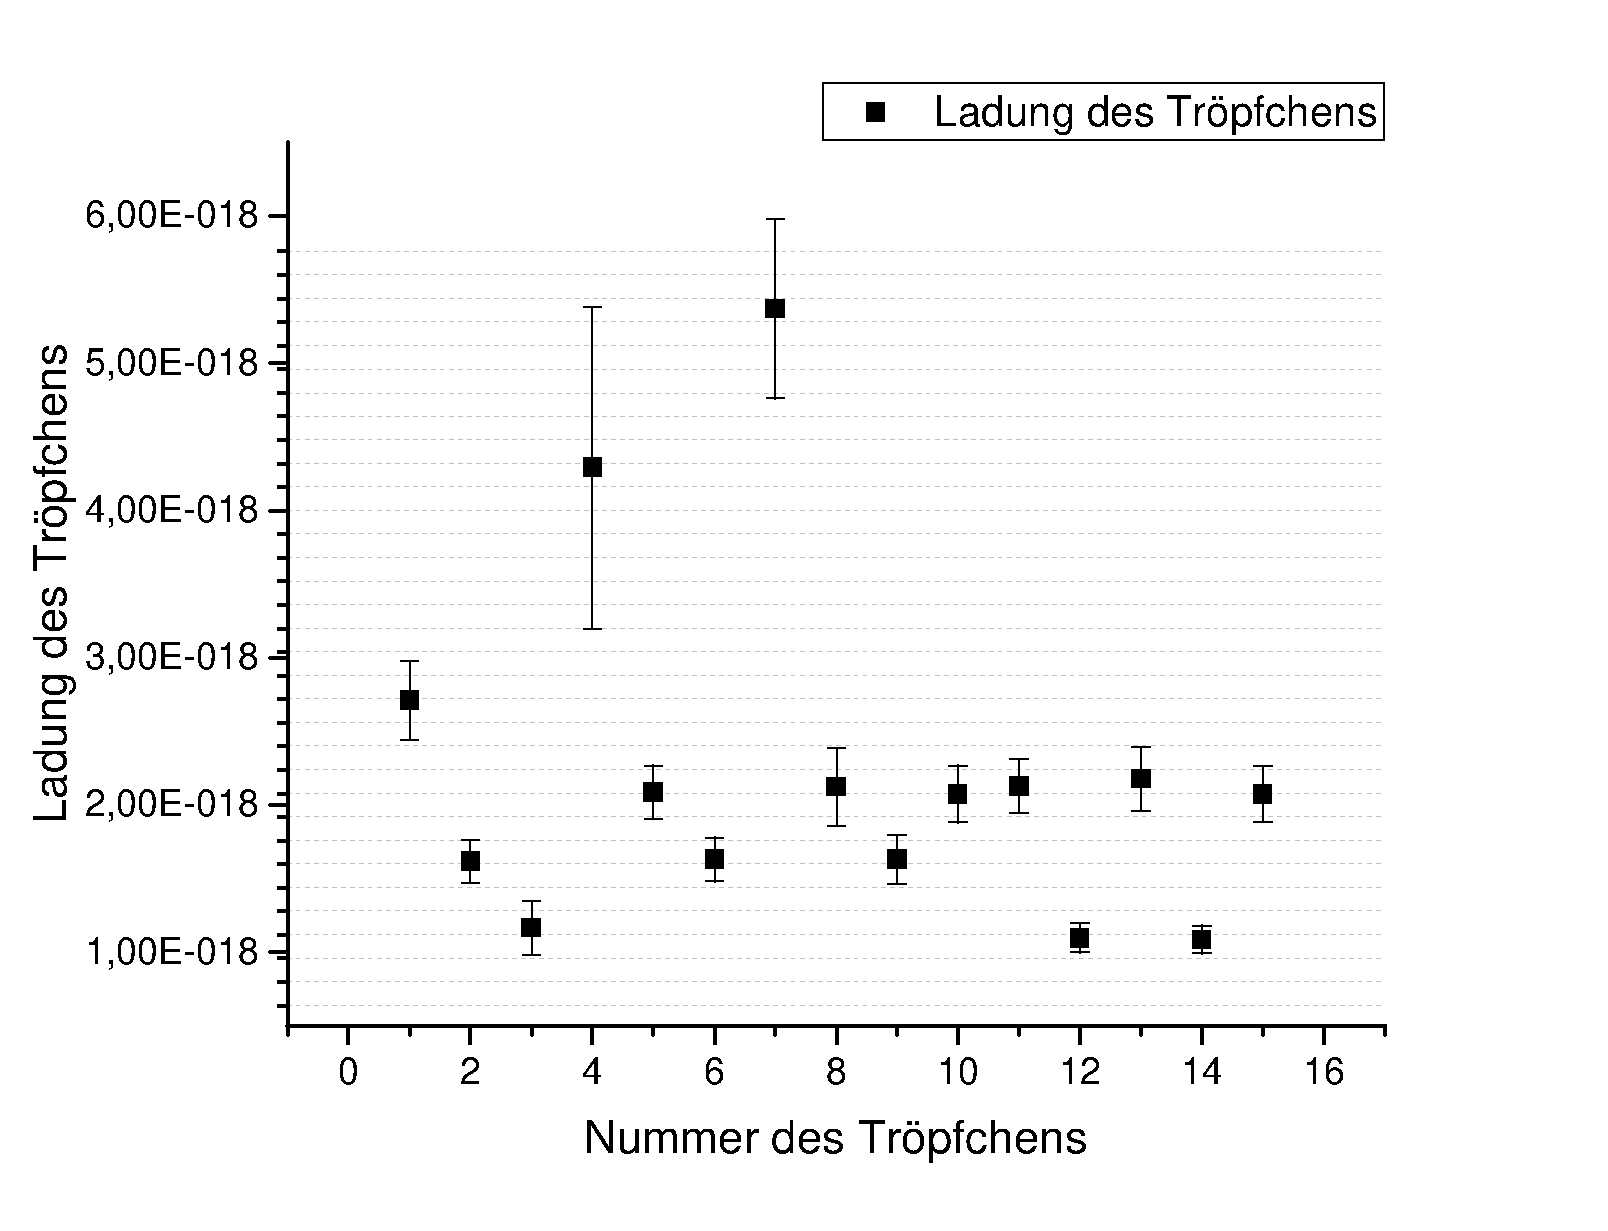
\includegraphics[width=1\textwidth]{Troepfchenladungen}
		\centering
		\caption{Die Ladungen, die sich gemäß \cref{Ladung} aus den Fall- und Steiggeschwindigkeiten der Tröpfchen ergeben. Die horizontalen gestrichelten Linien entsprechen dabei Vielfachen des Literaturwerts für die Elementarladung (vgl. \cite{Elementarladung})}
		\label{Tropf_Ladungen}
		\centering
	\end{figure} 
	

	%TODO Stokesscher Satz korrektur

	\subsection{Diskussion}
	%TODO Bezug/Nutzten oder sonst was
	%TODO auch hier die Hypothese wiederholen
	%TODO bezug auf unsicherheiten
	Wenn die Tröpfchengröße im Bereich der mittleren freien Weglänge der Luftmoleküle liegt, muss im Stokesschen Gesetz zur Reibung die Viskosität der Luft korrigiert werden.
	Da diese Cunningham-korrigierte Viskosität von dem Radius der Tröpfchen abhängt (die mithilfe der Viskosität berechnet wird), würde dies eine iterative, numerische Rechnung benötigen.
	Deshalb (und weil die Korrektur sehr gering ist) haben wir darauf bei der Berechnung der Ladung der Tröpfchen verzichtet.
	\par
	Der Literaturwert für die Elementarladung beträgt \SI{1,6021766208 \pm 0,0000000098 e-19}{C} \cite{Elementarladung}.
	In \cref{Tropf_Ladungen} sind die gestrichelten horizontalen Linien Vielfache der Elementarladung.
	Auffällig sind die Ausreiser Tröpfchen Nummer 4 und 7. 
	Beide weisen eine Unsicherheit von mehr als dem sechsfachem der Elementarladung auf. 
	Das dies der Fall sein würde bei einer zu hohen Ladung ist bereits aus den Vorüberlegungen bekannt.
	Die meisten Messwerte häufen sich um  eine Ladung von \SI{2,08e-18}{C}, da deren Unsicherheiten auch mehrere mögliche Vielfache der Elementarladung beinhalten, kann nicht gefolgert werden, dass die Ladung ein Vielfaches der Elementarladung ist.
	Die interessantesten Werte liegen bei \SI{1,12e-18}{C}, da sie die kleinsten Unicherheiten besitzen.
	Die Messpunkte 12 und 14 sind nahe an dem siebenfachen der Elementarladung, jedoch ist die Unsicherheit noch bei ca. \SI{1,602e-19}{C}.
	Es könnte also auch eine Ladung von $6,5 \cdot \SI{1,602e-18}{C}$ in den Öltröpfchen enthalten sein.
	Außerdem sind zwei Messpunkte mit einer genügend kleinen Unsicherheit unausreichend, um Schlüsse auf die Elementarladung ziehen zu können.
	

	Aus den von uns ermittelten Ladungen lässt sich die Elementarladung nicht bestimmen, ihre Existenz allerdings auch nicht ausschließen.

	
	\section{Schlussfolgerung}
	Das Experiment legt den Schluss auf die Existenz einer Elementarladung nahe, jedoch ist nicht ausgeschlossen, dass die gemessene Elementarladung das Doppelte der eigentlichen ist. 
	Durch mehrfaches Messen erkennt man allerdings,dass es keine Öltröpfchen mit einer Ladung kleiner als \SI{1,602e-19}{C} oder mit $(0.5+n)e$ gibt. 
	Folglich lässt sich erst durch ausreichend viele Messungen stochastisch die Existens einer Elementarladung bestätigen.
	Die 15 von uns gemessenen Tröpfchen lassen einen groben Schluss auf die Elementarladung zu, sind jedoch für eine genaue Bestimmung nicht genügend Messpunkte.

	Zusätzlich hätte man die Ladung auch durch ein genaues Einstellen der Spannung, sodass das Öltröpfchen schwebt, bestimmen können, dies ist aber unpraktisch, da die Spannung am Kondensator nicht ausreichend genau konfiguriert werden kann.
	Außerdem wäre nach wie vor der Radius des Tröpfchens durch eine andere Methode zu bestimmen.


	Eine mögliche Verbesserung des Experiments wäre die Bereitstellung einer stärkeren Spannungsquelle, sodass beispielweise auch ein Tröpfchen, das nur eine Ladung von $e$ und einen verhältnismässig großen Radius hat, aufsteigt.

	%TODO Rückgriff auf Hypothese und drittes Nennen dieser
	%TODO Millikan e/2 möglich  aber unwahrscheinlich
	%TODO nichts zu falsifizeiren
	
	%TODO Quellen zitieren, Websiten mit Zugriffsdatum
	%TODO Verweise auf das Laborbuch (sind erlaubt)
	%TODO Tabelle + Bilder mit Beschriftung

	\printbibliography
\end{document}
